%\documentclass[a4paper, 12pt, onecolumn]{scrartcl}
\documentclass{beamer}

%\usepackage{beamerarticle}
\usetheme{Darmstadt}
\beamertemplatenavigationsymbolsempty
\setbeamertemplate{footline}[frame number]

\usepackage[ngerman]{babel}
\usepackage[utf8]{inputenc}
\usepackage{amsmath}
\usepackage{amssymb}
\usepackage{graphicx}
\usepackage{siunitx}
\sisetup{per-mode=symbol}


\title{Bewegungen im 3D-Raum}
\author[Y. Jung]{Yvonne Jung}
\institute[HS Fulda]{Hochschule Fulda, FB AI}


\begin{document}

\frame{ \titlepage }

%\section*{Bewegungen im Raum}
\small

\begin{frame}{Weg-Zeit-Gesetz}
  \begin{itemize}
    \item Gleichmäßig beschleunigte Bewegung ($a = \text{const}$)
  \begin{equation}
    s (t) = s_0 + v_0 t + \frac{a}{2} t^2
  \end{equation}
    Mit Zeit $t$, Anfangsposition $s_0$, Anfangsgeschwindigkeit $v_0$\\
    Geschwindigkeit: $s' (t) = a t + v_0 = v (t)$\\
    Beschleunigung:  $v' (t) = a$
    
      \item Bsp. 1: Freier Fall \\
        Bewegung unter ausschließlichem Einfluss der Schwerkraft mit Fallbeschleunigung 
        $g = \SI{9.81}{\meter\per\square\second}$
      \begin{align}
        s (t) = \frac{g}{2} t^2
      \end{align}

      \item Bsp. 2: Schräger Wurf \\
        Kombination aus gleichförmiger Bewegung (d.h. $a = 0$) in Abwurfrichtung und freiem Fall
    
  \end{itemize}
\end{frame}

\begin{frame}{Kurven in Vektordarstellung}
  \begin{itemize}

        \item Bsp. 1: Gerade (für Parameter $t \in \mathbb{R}$)\\
      \begin{align}
        \vec{s} (t) = \vec{p} + t \vec{q}
      \end{align}
        \item Bsp. 2: Kreis (für $t \in [0, 2\pi]$)\\
      \begin{align}
        \vec{s} (t) = \left( \begin{matrix} \cos (t) \\ \sin (t) \end{matrix} \right)
      \end{align}
    
    \item Seien $\phi (t) , \psi (t)$ differenzierbar für $a \le t \le b$
    und $\vec{s} (t) = \left( \begin{matrix} \phi (t) \\ \psi (t) \end{matrix} \right)$
    Kurve mit $a \le t \le b$. Dann ist
      \begin{align}
        \vec{s'} (t) = \begin{pmatrix} \phi' (t) \\ \psi' (t) \end{pmatrix}
      \end{align}
    Tangentenvektor; d.h. $\vec{s'} (t)$ zeigt in Tangentenrichtung. \\
    Analog für 3D
    

\end{itemize}
\end{frame}

\begin{frame}{Bahnkurven}
  \begin{itemize}
    
    \item Sei $t$ Zeit und $\vec{s} (t)$ zeige auf Punkt in $\mathbb{R}^3$, der zur Zeit $t$
    durchlaufen wird. Dann heißt $\vec{s} (t)$ Bahnkurve.
    
    \item  Vektorielle Darstellung der Weg-Zeit-Fkt. $\vec{s} (t)$ im $\mathbb{R}^3$
    \begin{align}
    \vec{s} (t) = \vec{s_0} + \vec{v_0} \cdot t + \frac{1}{2} \vec{a_0} \cdot t^2 =
           \begin{pmatrix} s_x \\ s_y \\ s_z \end{pmatrix} + \begin{pmatrix} v_x \\ v_y \\ v_z \end{pmatrix} t + 
           \frac{1}{2} \begin{pmatrix} a_x \\ a_y \\ a_z \end{pmatrix} t^2
    \end{align}
    
    \item Übungsaufgabe (Wurfparabel)
    
    Ein Geschoss werde von einer Plattform in der Höhe $h = \SI{10}{\meter}$ über dem Boden mit einer Anfangsgeschwindigkeit 
    $v_0$ von $\SI{50}{\meter\per\second}$ in eine Richtung abgeschossen, die einen Winkel $\alpha$ von $40^{\circ}$
    mit der Bodenfläche bildet.
    
    \emph{(i)} Wie hoch fliegt es maximal? \\
    \emph{(ii)} Wie weit fliegt es?
  \end{itemize}
    
\end{frame}

\begin{frame}{Lösungsskizze Schräger Wurf}

    Annahme: Flugbahn liegt in $yz$-Ebene und $z$-Achse zeigt nach oben
    \begin{figure}[ht]
        \centering
            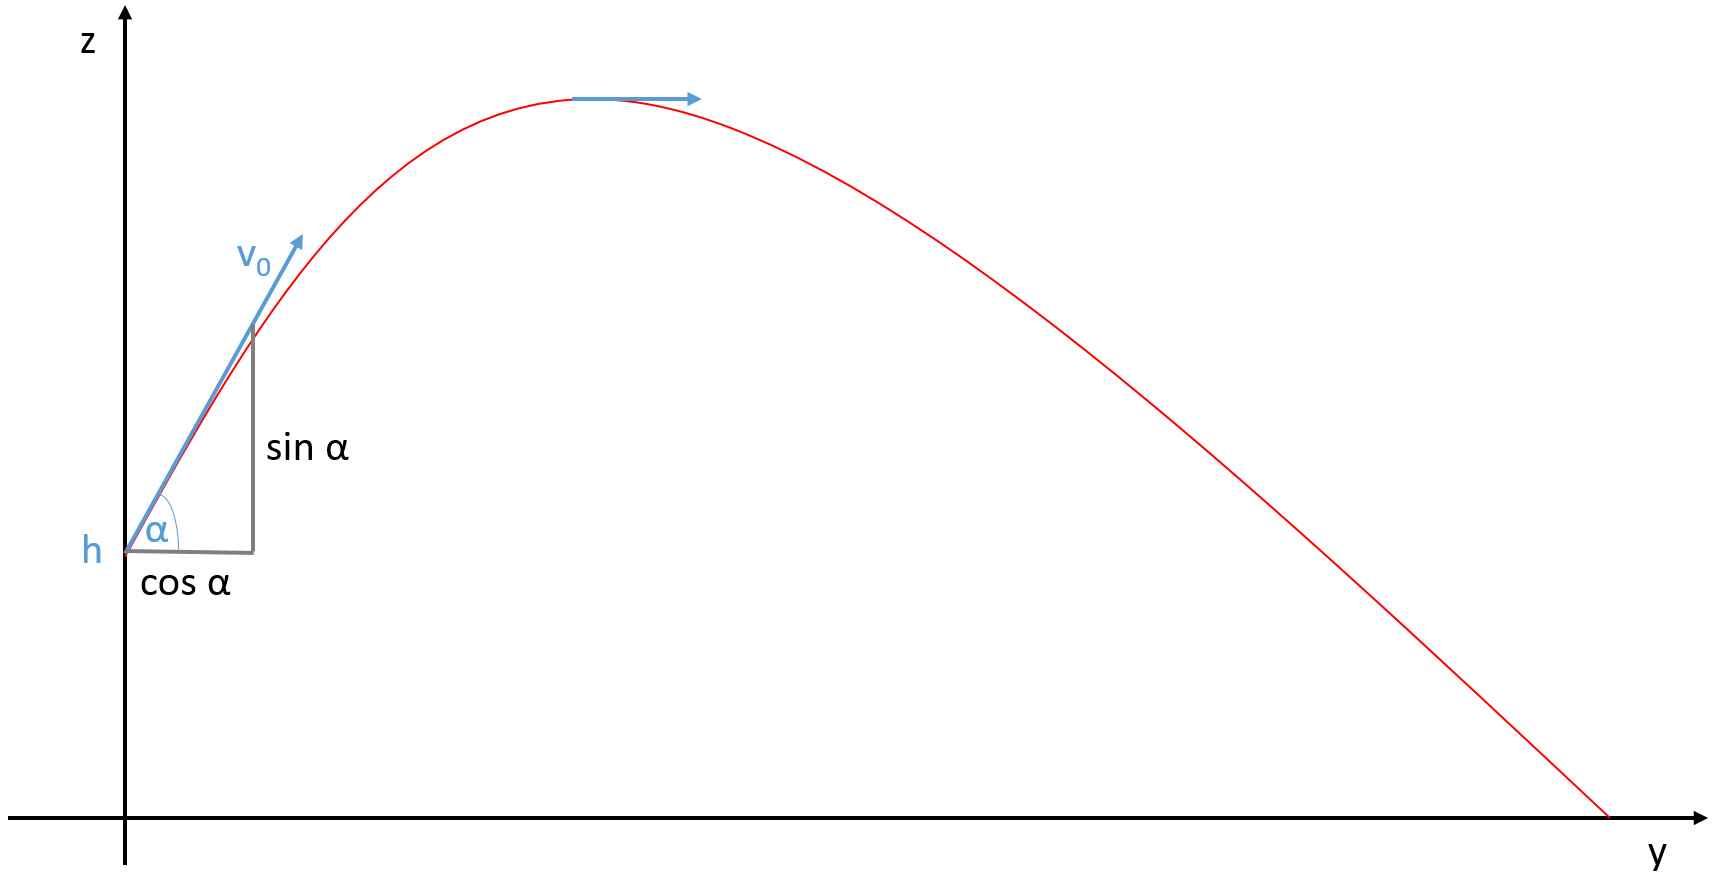
\includegraphics[width=1.0\textwidth]{flugbahn}
    \end{figure}

\end{frame}

\begin{frame}{Übungsaufgabe Schräger Wurf \emph{(i)}}
    
    \begin{itemize}
    \item Lösungsansatz für \emph{(i)}:
    
    Mit den Anfangsbedingungen
  \begin{align}
    \vec{s_0} = \begin{pmatrix} 0 \\ 0 \\ h \end{pmatrix},
    \vec{v_0} = v_0 \begin{pmatrix} 0 \\ \cos \alpha \\ \sin \alpha \end{pmatrix},
    \vec{a} = \begin{pmatrix} 0 \\ 0 \\ -g \end{pmatrix},
  \end{align}
    wobei $\vec{v_0}$ aus den trigonometrischen Beziehungen (Steigung) folgt,
    ergibt sich folgende Bahnkurve:

  \begin{equation}
    \vec{s} (t) = \begin{pmatrix} x (t) \\ y (t) \\ z (t) \end{pmatrix} =  
    \begin{pmatrix} 0 \\ 0 \\ \SI{10}{\meter} \end{pmatrix} + 
    \SI{50}{\meter\per\second} \begin{pmatrix} 0 \\ \cos 40^\circ \\ \sin 40^\circ \end{pmatrix} t + 
    \frac{1}{2} \begin{pmatrix} 0 \\ 0 \\ \SI{-9.81}{\meter\per\square\second} \end{pmatrix} t^2
  \end{equation}

    \end{itemize}
\end{frame}

\begin{frame}{Übungsaufgabe Schräger Wurf \emph{(i)}}
    \begin{itemize}

    \item Maximale Höhe $h_{max}$ (Extremum) ist genau dann erreicht, wenn Ableitung 
    der Funktion $z (t)$, welche die Höhe bestimmt, Null wird: \\
    $z (t) = h_{max} \Leftrightarrow z' (t) = 0$

  \begin{eqnarray}
    z (t)  &=& \SI{10}{\meter} + \SI{50}{\meter\per\second} \cdot \sin 40^\circ \cdot t - 
        \frac{\SI{9.81}{\meter\per\square\second}}{2} \cdot t^2 \\
    z' (t) &=& \SI{50}{\meter\per\second} \cdot \sin 40^\circ - \SI{9.81}{\meter\per\square\second} \cdot t \stackrel{!}= 0
    \label{eq:zStrich}
  \end{eqnarray}

    Auflösen von Gleichung \ref{eq:zStrich} nach $t$ ergibt für den allgemeinen Fall 
    $t = \frac{v_0 \cdot sin \alpha}{g}$ \\
    Eingesetzt in $z (t)$ ergibt sich hier für $h_{max}$ ungefähr $\SI{62.6}{\meter}$
    
    \item Rechnet man alternativ mit $\alpha = 70^{\circ}$ erhält man eine Maximalhöhe von etwa $\SI{122.5}{\meter}$
    
    \end{itemize}
\end{frame}

\begin{frame}{Übungsaufgabe Schräger Wurf \emph{(ii)}}
    \begin{itemize}
    
    \item Lösungsansatz für \emph{(ii)}:
    
    Die maximale Wurfweite ist erreicht, wenn das Geschoss wieder am Boden ist, 
    es also gilt: $z (t) = 0$ (mit  $t \ge 0$)
    
    Da $z (t)$ eine quadratische Gleichung der Form $t^2 + p t + q = 0$ ist,
    kann der Parameter $t$ über die \emph{p-q-Formel} bestimmt werden mit \\
    $t = -\frac{p}{2} \pm \sqrt{\frac{p^4}{4} - q}$
    
    Hat man so Zeit $t$ bestimmt, für die $h = \SI{0}{\meter}$ ist, muss
    man diese in $y (t) = v_0 \cdot \cos \alpha \cdot t$ einsetzen, um  
    Gesamtflugweite zu bestimmen
    
    In unserem Bsp. sind das ungefähr $\SI{262.4}{\meter}$ in $y$-Richtung
    
    
    \item Modifiziert man Aufgabenteil \emph{(ii)} so, dass nur gefragt wird, wie weit das Objekt 
    fliegt, bis es wieder die Ausgangshöhe von $\SI{10}{\meter}$ erreicht hat, dann
    erhält man für $t$ die doppelte Zeit bis zum Erreichen der Maximalhöhe erhält, 
    d.h. $t = \frac{2 v_0 \cdot sin \alpha}{g}$
    
    Eingesetzt in $y (t)$ ergibt sich für die Flugweite nun ca. $\SI{251}{\meter}$
    
    \end{itemize}
    
\end{frame}

\begin{frame}{Kräfte}
    
  \begin {itemize}
    \item Grundgleichung der Mechanik \\
    (2. Newton'sches Axiom)
  \begin{align}
    \vec{F} = m \cdot \vec{a}
    \label{eq:fma}
  \end{align}
    mit $m = \text{const}$ und $[F] = \frac{kg \cdot m}{s^2} = N$
    
    \item Wirken gleichzeitig $n$ Kräfte, z.B. Gewichtskraft $F_G = m \cdot g$ etc.,
    dann gilt für die Gesamtbeschleunigung $\vec{a} (t)$
    \begin{align}
    \sum_{i=1}^{n} \vec{F_i} (t) = m \cdot \vec{a} (t) = m \cdot \vec{s''} (t)
    \end{align}
    
    \item Tipp: Einheiten-Check nicht vergessen! Stimmen die berechneten Einheiten
    nicht, kann das Endergebnis nicht richtig sein
    
    \end{itemize}
    
\end{frame}

\begin{frame}{Differentialgleichungen}
    
    \begin {itemize}
    
    \item  Eine Gleichung der Form $f(t, s, s', s'', ..., s^{(n)}) = 0$ heißt gewöhnliche 
    Differentialgleichung (DGL) $n$-ter Ordnung (engl.: ODE) \\
    Jede Fkt. $s (t)$, die die DGL löst, heißt Lsg. der DGL
    
        \item Anfangswertproblem (AWP)\\
        Geg. durch Anfangsbedingungen $s^{(k)} (a) = \alpha_k$ für $k \in \{0, 1, ..., n\}$
        
        \item Euler'sches Polygonzugverfahren\\
        Einfachste numerische Lösungsmethode eines AWP durch Approximation mit Tangente 
        (Gleichung \ref{eq:tan})
        
        \item Achtung: Euler-Verfahren wird schnell \emph{instabil}, wenn Schrittweite $\Delta t$ zu groß, 
        da es sich aus Taylorreihenentwicklung 1. Ordnung (lineare Näherung) ableitet
        
        \begin{itemize}
        \item Verbesserungen z.B. mit Runge-Kutta oder Verlet-Integration
        \end{itemize}
   
   \end{itemize}
\end{frame}

\begin{frame}{Euler-Integration}
   \begin{itemize}
        \item \emph{(I)} Geg.: DGL $s' = f (t, s)$ mit Anfangsbed. $s (t_0) = s_0$ und 
        Schrittweite $h$ mit $h = t_{n+1} - t_n$
        
        \begin{eqnarray}
                    s'      &=& \lim_{h \rightarrow 0} \frac{s (t + h) - s (t)}{h}
                                \approx \frac{s (t + h) - s (t)}{h} \\
        \Rightarrow s_n'    &=& \frac{s_{n+1} - s_n}{h} \stackrel{!} = f (t_n, s_n) \\
        \Rightarrow s_{n+1} &=& s_n + h \cdot f (t_n, s_n) \label{eq:tan}   % Tangente
                  % s_0     &=& s (t_0)
        \end{eqnarray}
        
        \item \emph{(II)} Geg.: DGL $s'' = f (t, s, s')$ mit Bed. $s (t_0) = s_0$ und 
        $s' (t_0) = v_0$ \\
        Setze $v (t) = s' (t) \Rightarrow v' (t) = f (t, s, v) \stackrel{!}= a (t)$
        
        \begin{eqnarray}
        v_{n+1} &=& v_n + h \cdot f (t_n, s_n, v_n) \label{eq:v}\\   % Tangente
        s_{n+1} &=& s_n + h \cdot v_n \label{eq:s}
        \end{eqnarray}
        mit $s_0 = s (t_0)$, $v_0 = v (t_0)$ und $a_n = f (t_n, s_n, v_n)$
        
   \end{itemize}
\end{frame}

\begin{frame}{Partikelsysteme}
   \begin{itemize}
        
        \item Partikel hält Zustandsvariablen $\vec{s}$ und $\vec{v}$ für aktuellen Zeitschritt $t$
        
        \item Auf Massepartikel $p$ wirken verschiedene Kräfte $\vec{F_i}$\\
        Daraus folgt wegen Gl. \ref{eq:fma} $\forall p$ für aktuelle Beschleunigung $a_n$
        \begin{align}
        \vec{a_p} (t) = \vec{s_p''} (t) = \frac{\sum{\vec{F_i}}}{m_p}
        \end{align}
        
        \item In Zeitschritt-Schleife werden je neue Position $s_{n+1}$ und neue Geschwindigkeit $v_{n+1}$
        mit Hilfe der Gleichungen \ref{eq:s} und \ref{eq:v} berechnet
        \begin{eqnarray}
        v_{n+1} &=& v_n + \Delta t \cdot a_n\\
        s_{n+1} &=& s_n + \Delta t \cdot v_n
        \end{eqnarray}
        
        \item Dabei wird die zuvor über alle einwirkenden Kräfte 
        bestimmte Beschleunigung $a_n$ in Gleichung \ref{eq:v} eingesetzt
    
       \end{itemize}
\end{frame}

\begin{frame}{Masse-Feder-Systeme}
   \begin{itemize}

    \item Z.B. zur Simulation von Kabeln, Haaren oder Kleidung
    \item Nachbarpartikel sind miteinander verbunden\\
    Verbindung wird modelliert durch Federn (i.d.R. mit Dämpfung)
    
    \item Hooke'sches Gesetz\\
    Schwingung beim Federpendel (Federkonstante $D$)
    \begin{align}
    \vec{F} (t) = -D \cdot \vec{s} (t)
    \end{align}
    Mit $\vec{s} (t)$ -- gesucht -- Auslenkung zur Zeit $t$

    \item Dynamisches Kräftegleichgewicht beschrieben durch DGL
    \begin{align}
    m \cdot \vec{a} (t) = -D \cdot \vec{s} (t) \Rightarrow \\
    \vec{s''} (t) + \frac{D}{m} \cdot \vec{s} (t) = \vec{0}
    \end{align}
    
    
  \end{itemize}
\end{frame}

\vfill
\bibliographystyle{geralpha}
\begin{thebibliography}{Len12}
\bibitem[Len12]{Lengyel}
{\normalfont\scshape Lengyel, Eric}: {\em Mathematics for 3D Game Programming and Computer Graphics (Third Edition)}.
\newblock Cengage Learning, Boston, MA, USA, 2012.
\end{thebibliography}

\end{document}
